\documentclass{article}

\usepackage{multirow}
\usepackage{longtable}
\usepackage{amsmath}
\usepackage{graphicx}
\usepackage{float}
\usepackage{array}
\usepackage[a4paper, total={15cm, 24.5cm}]{geometry}

\title{Computing Infrastructure}
\author{Elia Ravella}
\begin{document}
	\begin{titlepage}
		\maketitle
	\end{titlepage}
	
	\tableofcontents
	\clearpage
	
	\clearpage \part{Introduction}
		\section{Computing Infrastructure}
			What is a CI? A CI is a \emph{technological structure} that provides hardware and software for computation to other systems. This means a lot: is a joint (and heterogeneous) system that comprises both HW and SW to deliver several services. With CI is not intended the \emph{application delivered} but the combination of elements that makes the application available and running.\\
			So everything in between a RaspPI that does torrent seeding from a local network to the whole datacenter that runs an AWS service can be considered a computing infrastructure.
			
	\clearpage \part{Hardware Infrastructures}
		\section{Data Centers}
			\subsection{Pros and cons}
				Data centers are big centralized CIs that comprise a lot of servers (to provide computations) a communication infrastructure, and a storage service.\\ 
				PROS of a DC:
				\begin{itemize}
					\item Lower IT cost: renting a virtual machine is cheaper than buying / building and maintaining a whole system (for some time horizons, of course);
					\item High performance: virtualized resources make scaling easier, and provides optimized and finely tuned services that an in-house solution cannot provide \emph{so} easily and fast;
					\item No effort software updates;
					\item Unlimited (!) storage capacity;
					\item Increased data reliability;
					\item Universality of accesses;
					\item Device indipendence.
				\end{itemize}
				The CONS of a DC can be found simply inverting the POV for the PROS aspects: outsourcing resources gives "someone else" the control over some crucial aspects of a CI. This is a good thing when costs (also time costs) must be reduced, but can be a bad thing when a fine grained control over a full system is needed. Also, \emph{latency} pops in, due to the needed connection to the DC.
				
			\subsection{DCs ans WSCs}
				The data center approach has been emerging in the last years. The idea behind it is that we should not "overpack" nodes of a network with all the computing capabilities required, but instead giving them a connection to such CIs. Data centers are the perfect example for this paradigm: the user interact with a client (that can be \emph{any kind of device}) that also interact with a remote structure to provide computations. To a careful watch, SaaS and their spread are a direct conseguence of this paradigm shift. Another use of DCs is using their computing capabilities not in a fragmented way to provide miriads of services, but to perform an \emph{extremely costly computation}, like a training of a neural network.\\
				From a DC approach we are moving to Warehouse Scale Computers nowadays. This latter approach consists of NOT "mixing up the pot" in a DC (so having a lot of heterogeneous technologies in order to achieve different tasks) but instead to "homogeneify" the cloud structure in order to do better optimization of it. Not only in the HW, but also in the SW. To centralize the DC capabilities under a single organization (as often happens) means that clients no more run their application on someone else's hardware, but instead choose from a set of precooked solutions by such vendor/organization. Is this \emph{bad}? WSCs are just a "SaaS - oriented" Data Center Architectures, so \emph{there's no real transition between DCs and WCSs} the only transition is in the number of \emph{virtualiazed layers the client must go through to access an application}.\\
				We can sum up the difference between DCs and WSCs in this way: where DCs are intended as a powerful collection of different servers, WSCs tries to offer a homogeneous interface that can be used also as a single server to such a collection of hardware. Still, if we consider a larger definition for DCs, WSCs are a type of DCs. 
				\begin{figure}[H]
					\centering
					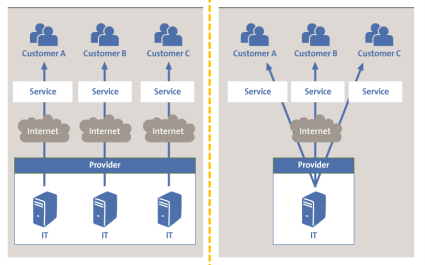
\includegraphics[width = \textwidth]{./images/wsc.png}
					\caption{Left, the classic DC approach. Right, the WSC scheme.}
				\end{figure}
				
			\subsection{Architectural Overview of DCs and WCSs}
				A standard data center building is organized in separated modules, every one dedicated to a specific task. The four main modules types are
				\begin{itemize}
					\item Servers: computations
					\item Storage
					\item Networking: intended as the whole communication infrastructure
					\item Building-integrated systems:
						\begin{itemize}
							\item Cooling system: often as powerful as the server themselves, fundamental for getting rid of excess heat
							\item Power supply: integrated in the building and provided with systems to avoid power shortage
							\item Failure recovery: physically realized as a building module in order to be as most fault - tolerant
						\end{itemize}
				\end{itemize}
				Servers are organized in racks, blades or tower, and are the classical computational unit usually found in server farms. They could also not have memory attached.\\
				Storage is the crucial long term memory for a CI. Usually built with flash SSDs and ferromagnetic mechanical disks. The memory units must provide high speed I/O capabilities, and also advanced networking power, also at software level (NAS, SAN, DAS).\\
				The networking infrastructure is the backbone of the communication in (and from/to) a data center. Structured hierarchical approach to networking structures and organization are used to ensure security and performace\\
				The building itself is part of the CI.\\
				Next sections will delve into the details of the single modules.
			
			\subsection{Servers}
				Servers are the computational compartment of a WSC. They're organized in racks (shelves) that host the computational units (pizza box computer). Servers are just computers. That's all. They got a MOBO, local primary memory, a CPU, and I/O capabilities. They can be organized as
				\begin{itemize}
					\item Towers: cheap, cooling is easy, upgrade is easy. They're also big, and they provide low density of computational power.
					\item Blades: also called hybrid racks, the idea is similar to the rack system, but a server is inserted \emph{vertically} instead of \emph{horizontally} in a dedicated place. This (together with the average smaller size of a blade server) enhances computation per volume ratio while keeping all the pros of a rack system. Blade servers have disadvantages: heat management is complex, and enclosures and envelops are more expensive wrt racks.
					\item Racks: literal racks that host the pizza box shaped computational units, and accomodate all the wiring and additional connection or cooling systems. They can host also heterogeneus components, not only standard computational modules. Rack's dimension and geometry is a standard. Rack organization provides better failure handling and simplified cable management, but they're more power demanding (wrt towers) and mainteinance is a mess (mmultiple devices must be maintained at the same time).
				\end{itemize}
				To sum up:
				\begin{center}
					\begin{tabular}{ | m{2cm} || m{5cm} | m{5cm} |}
					\hline
					\textbf{Format} & \textbf{Pros} & \textbf{Cons} \\
					\hline
					\hline
					Tower & Cost effective, easy to cool down (low component density), easy to upgrade & bulky, not so powerful, messy cable management \\
					\hline
					Rack & Easy to replace, straightforward cabling, cost effective & high component density leads to high power consumption, difficult to maintain singularly \\
					\hline
					Blade & Super compact, support for centralized management, easy cabling & Expensive first configuration, nightmare to cool down \\
					\hline
					\end{tabular}
				\end{center}
				
				\subsubsection{Hardware Accellerator}
					WSCs architectures and the rise of heavy computation loads (like for intense machine learning and AI training) have caused a spike in the complexity required every computation, even far beyond the Moore's law. To satisfy this need, dedicated hardware (in the form of \emph{hardware accellerators}) are deployed in WSCs, to enhance the performance in determined fields.
					
					\paragraph{GPU}
						Graphical Processing Units are featured in accellerators to enhance \emph{parallel fast computation}. Due to the architecture of them, they're also perfect to do matrix computation. 
						
					\paragraph{TPU}
						Tensor Processing Units. These are more specialized GPUs in the machine learning direction. They're (simplifying) custom circuits to support tensor computations (matrix calculus) that are \emph{very fast} at doing so. Google released TPUv3 at the time I'm writing
						
					\paragraph{FPGA}
						Good ol' Field Programmable Gate Array circuits are still used to enhance performance in custom computational oriented architectures. These circuits are somewhat "fully customizable" hardware computers that if programmed in a very specific way can enhance \emph{every kind} of possible computation. 
			
			\subsection{Storage}
				Storage. Not much more. Technologies involved: HDDs and SSDs and Flash memory. Performance (and relevant) parameters:
				\begin{itemize}
					\item read / write speed and latency (or seek time)
					\item memory density
					\item security: but this is intended as an hardware security, not data security (for now)
					\item cost
				\end{itemize}
				
				\subsubsection{Storage Systems - DAS, NAS, SAN}
					\begin{itemize}
						\item Direct Attached Storage is every device that offers storage capabilities and is directly attached to the unit processing such data in the storage. HDDs are DAS for personal computers, for example. They're directly accessible from the OS of the machine accessing it. They're difficult to scale. They are difficult to manage when particular storage solutions are needed. Moreover, the OS's proprietary file sharing model / protocol / software must be used in order to share files with other machines.
						\item Network Attached Storage is a storage system that lies \emph{on the other end} of a network. A NAS only offers data services accessible from dedicated protocols (as FTP, SAMBA) and it's \emph{an actual computer} that offers services. A NAS is a \emph{full fledged computer} that's \emph{only meant for storage services}, accessible through network protocols. It's located somewhere in the network. It's easily scalable (both augmenting the storage of a single NAS or multiplying the NAS number work).
						\item Storage Area Network is like NAS, but the remote storage unit are \emph{passive} and are directly accessible by the OS (by means still of a network connection). They're \emph{remotely accessed simple storage devices}. Disks are visible \emph{like local storage, like DAS} to the server machina, but they're network attached. They have specialize hardware that mask the network in between, and the SAN can be accessed \emph{directly through the filesystem}. 
					\end{itemize}
					\begin{figure}[H]
						\centering
						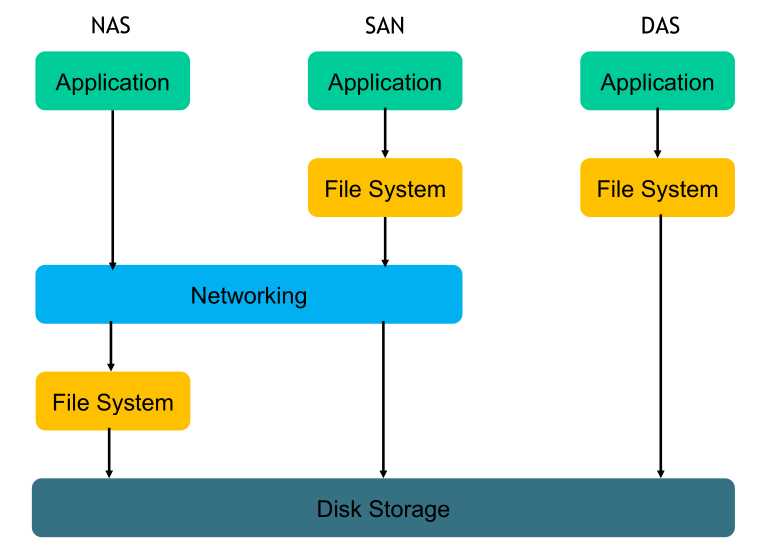
\includegraphics[width = \textwidth]{./images/storage.png}
					\end{figure}
					
			\subsection{Networking}
				Design a network architecture for a WSC ain't easy job. Moreover, the actual networking technologies haven't a straightforward horizontal scaling solution. This means that the \emph{the number of connections needed increases exponentially with the number of clients}, except for some clever solutions, if we are looking for a capillar connectivity. And, ina WSC, we are. Our aim is to provide additional \underline{bisection bandwidth}, that's the bandwidth available between two partitions of the network.\\ 
				A WSC networking system can be divided in 2 separate blocks:
				\begin{itemize}
					\item an internal LAN that connects all the components (the servers) among themselves
					\item an interface to the internet (DMZ..?)
				\end{itemize}
				
				Obviously, the networking infrastructure in a WSC is crucial because it also connects the functional units (as the server) to the storage infrastructure and so it's \emph{fundamental} that this connections is solid. The need of inter-server bandwidth incerases exponentially with the number of server, obviously.\\
				A WSC internal network is usually divided in 3 levels:
				\begin{enumerate}
					\item Access: this network layer is the one that connects the servers to the network. It's embodied by the network infrastructures embedded in the server racks.
					\item Aggregation: this level groups the servers together (VLAN-like) and it's usually implemented as Top Of the Rack switches, that group together all the server in a aisle (for example).
					\item Core: furthest level from the single server, aggregates entities of the "aggregation" level.
				\end{enumerate}
				Many network topologies are out there:
				\begin{enumerate}
					\item Fat tree (classic hierarchical topology, clearly visible access aggregation and core levels
					\item D-Cell, recursive topology. Cells are organized in levels and the network "builds itself" through a discover mechanism
					\item Hypercube topologies
				\end{enumerate}
				
			\subsection{Building and Non-IT Equipment}
				The way in which the hardware is arranged \emph{inside} a DC is as crucial as the building composing the DC itself, as well as the non-IT instruments (like the cooling system, or the energy system) that completes the DC structure.\\
				
				\subsubsection{Energy System}
					Powering a DC is difficult on many layers; first of all, computing infrastructures of this scale need a lot of energy, but this energy must be provided steadily and must be always available. Moreover, the power must not be subject to cuts, improvised shortages or outing. So not only the energy system of a DC must handle a lot of power, but should also handle it \emph{with care}. Usually, DCs have a UPS that does all this work.
					
					\paragraph{The UPS}
						The Uninterruptible Power System is the hearth of the energy subsystem of a datacenter. It is composed of 3 main parts:
						\begin{enumerate}
							\item A socket to the external provided power. This is usually high voltage power that must be trimmed down (order of 50 kV) in order to be utilized.
							\item An internal generators system that is powered up when the external power supply fails. These systems takes usually 10 to 20 seconds to power up.
							\item A battery array to bridge the gap between an external power outage and the wind-up time of the backup generators.
						\end{enumerate}
						The UPS must also "filter" the external power provided, cutting spikes and removing dangerous armonics in current. This is usually done by a AC to DC to AC converter. Then, electric power is sent to power distribution units (that resembles the one in the houses) that manages the power flow in each row or rack.
				
				\subsubsection{Cooling System}
					The cooling system removes the heat generated by the equipment. It must imply some sort of loop (thermodinamically speaking) that warms up a medium and then transfers the heat somewhere else.\\
					There are several strategies to cool down a data center:
					\begin{itemize}
						\item Open loop: the fresh air is "sucked in" from the outside and then passively heated by the servers themselves. The hot air exhaust is let flow out from the top. In fact, this is a open-the-windows approach. Obviously this approach is very easy to set up, and requires little to no additional hardware (the additional hardware can be needed to cool down the air intake, or speed up the airflow, controlling humidity...) and can perform very well for its cost. Being so simple, it has its drawbacks: it depends from the outside temperature, the air flow is "uncontrolled"...
						\item Closed loop: this approach is more similar to the personal computer's one. Heat is removed from the hardware and then the medium used to remove it is chilled in another place. Why closed? Because it does not depends on external air / chiller medium to refrigerate a room. Instead, the medium is chilled in a heat exchanger (usually located in a dedicated CRAC room) and then reinsterded in the loop. Multiple loop can be exploited in order to enhance the control over the heat transfer.
						\item In rack cooling: manufacturers of server racks can add a device that acts as a heat exchanger (in particular, generally it's a air to water exchanger) that sucks out the out directly from the servers.
						\item In row cooling: as in rack cooling, just done at row level.
						\item Circuit cooling: as in a personal PC, we can directly cool down circuitery (usually with liquid cooling systems) and this approach offers the most elevated performaces. However, liquid circuitery cooling system are hard to manage, other than inpractical.
					\end{itemize}
					
				\subsubsection{DCs Tiers}
					Availability of a DC is expressed on a scale, from one to four, that depends on a set of fixed parameters. Here's the table:
					\begin{figure}[H]
						\centering
						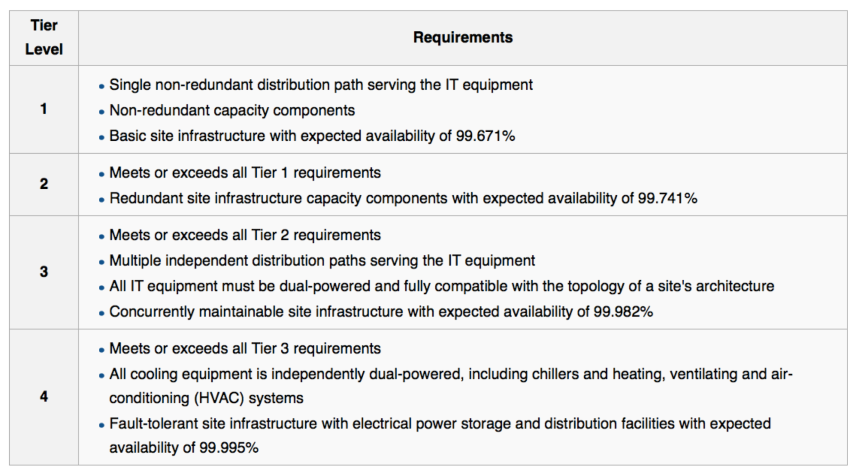
\includegraphics[width = \textwidth]{./images/tiers.png}
						\caption{DC tiers}
					\end{figure}

	\clearpage \part{Software Infrastructure}
		\section{Virtualization}
			Virtualization is the procedure of "making a resource available through software artifacts". This resource can range from a particular kind of processor to a whole application set or service. Virtualization is the main technology enabling cloud computing, because of the flexibility mainly, the isolation and the security offered. Server VMs are implemented without using a host OSs as the personal computer one, they rely instead on a virtual machine monitor (like HyperVisor) that manages the hardware to run multiple VMs at the same time.
			
			\subsection{Virtual Machines}
				A machine is defined as "execution environment capable of running a program". This is a very general definition, that ranges from washing machines to computing infrastructures for neural network training. A virtual machine differs from a physical machine by the way in which hardware is managed. A physical machines handles hardware by the OS, while a VM has to interface with a hardware supervisor in order to access it. "Formally", a VM is a \emph{logical abstraction able to provide a virtualized execution environment}.\\
				A VM must provide identical software behaviour (execution on a VM should be transparent). The VM, being composed of a mix of hardware and virtualizing/virtualized software, usually has worse performance wrt his physical counterimplementation. The VM is in charge of the translation of the virtualized software instructions into effective machine instructions. 
	
			\subsection{Levels of Virtualization}
				Given the intrinsically layered structure of an operating system, it's easy to discriminate between virtualizatiion approaches basing on the layer they address.
				\begin{figure}[H]
					\centering
					\begin{minipage}{0.45\textwidth}
						\centering
						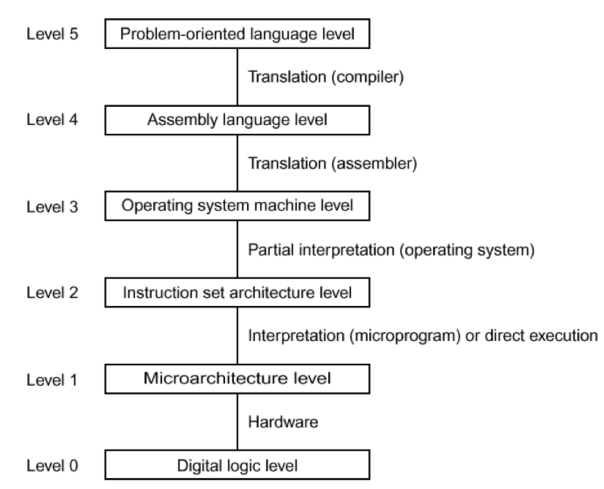
\includegraphics[width=0.9\textwidth]{./images/layers.png}
						\caption{The layered operating system structure}
					\end{minipage}\hfill
					\begin{minipage}{0.45\textwidth}
						\centering
						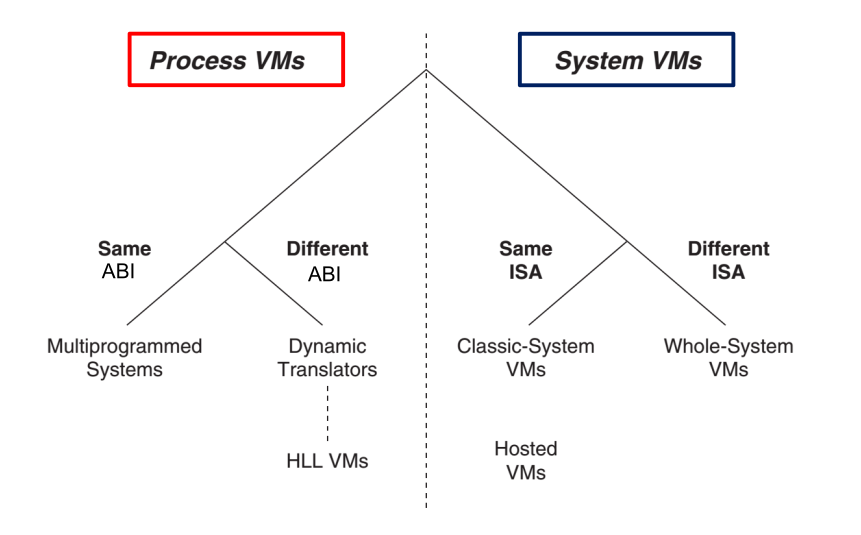
\includegraphics[width=0.9\textwidth]{./images/vms.png}
						\caption{VMs and what they virtualize}
					\end{minipage}
				\end{figure}
				
				\subsubsection{Multiprogrammed Systems}
					Far left of the schema, and it's just a classic parallel OS. It's arguable it is a real VM, because all the traditional hardware-sharing computations nowadays exploit this model. 
					
				\subsubsection{High Level Language Virtual Machines}
					Java approach; isolated execution environment for each application. The VM just translates from the proprietary binaries to the actual machine's executable code. "Code once run everywhere".
					
				\subsubsection{System VMs}
					Virtual machine monitor on the bare metal, carries out the sharing. Virtual machine's on top of the VMM, and when a hardware-call is done this is passed through the VMM. The VMM uses the same ISA (the one of the machine). VMM can also be a program installed in another OS: in that case we're talking about \emph{whole system VMs}\footnote{Virtualbox approach}.
				
			\subsection{Virtualization Implementation}
				As already said, in order to virtualize something we have to add some middleware in the software stack that carries out the virtualizing mechanism. We can put this layer \emph{between the hardware and the OS}, or \emph{between the operating system and the processes} as in JVM or even \emph{between the OS and other OSs}, as in virtualbox.\\
				As a remainder, a virtualization software should provide
				\begin{itemize}
					\item Partitioning between softwares
					\item Isolation, so fault tolerance and security
					\item Encapsulation: the state of a VM can be easily stored and moved
					\item HW indipendence. As incapsulation, but for the whole execution
				\end{itemize}
			
			\subsection{VMM}
				We use three terms to define the same thing: Virtual Machine Manager, Virtual Machine Monitor and HyperVisor. They're the same thing, so \emph{a piece of software dedicated to virtualize stuff}.\\
				Hypervisors are the software that acts directly attached to the machine hardware and are capable of hosting an OS.
				\begin{itemize}
					\item Type 1 hypervisors provide an abstraction and a full environment to a host relying directly on the hardware.
					\item Type 2 hypervisors (virtualbox) provide the virtualized hardware exploting \emph{a host operating system}.
				\end{itemize}
				\begin{figure}[H]
					\centering
					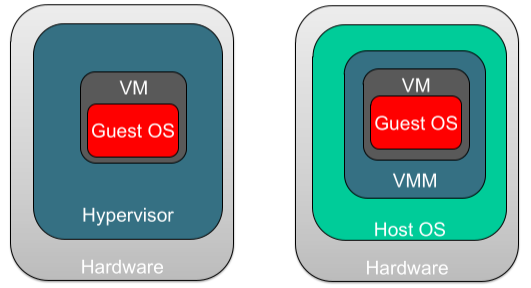
\includegraphics[width = \textwidth]{./images/VMMs.png}
					\caption{Type 1 and type 2 VMMs}
				\end{figure}
				
				\paragraph{Paravirtualization}
					A paravirtualized system \emph{can in certain conditions bypass the hypervisor and directly access the hardware}. This is done to improve performance: certain operations (depending from the OS, the hardware and the hypervis itself) are infinitely slower if run in the virtualized domain. A paravirtualized solution would execute these operations directly on the hardware, eventually "trapping" some execution paths. Paravirtualized systems offers increased performance and slimmer VMM, but the guest OS must be explicitly ported to the para-API.
				
			\subsection{Containers}
				A container is a pre configured package that comprises all the software pieces needed to run a particular type of software (like the database, the support for certain languages and services). All the software comes \emph{configured}. This approach does not fall entirely under the "virtualization" hat, because they do not depend on a OS (the container does not provide one). Instead, they rely on a container engine (as the Docker engine).
				
		\section{Cloud Computing and Edge/Fog Computing}
			Virtualization paved the way to intensive cloud computing. Being able to virtualize a resource means to \emph{have it available and accessible all the time}\footnote{That's a bold statement. But with the right approximations, seems legit.}. It also decouples the hardware and the software.\\
			One of the most used configuration aims to consolidate the usage of a single server, providing a dedicated environment \emph{for each app} and they can all run in the same machine. This is a huge improvement wrt "an app for each server". On top of the hypervisor software we can also build a \emph{distributed VM Monitor} that handles multiple VMs \emph{across a cluster of machines}: this improves load balancing, perfomrmance and \emph{resource usage}.\\
			
			\subsection{Cloud Computing and Services}
				Cloud computing is a model for enabling on demand network access to a shared pool of computing resources. The cloud approach pushed the *aaS paradigm to his limits: it started as "outsourcing to someone in the internet some computations" and it's "giving someone in the internet full control over our technologic stack".
				
				\subsubsection{Software as a Service}
					Software as a Service is the mechanism that allows users to access an entire software (an entire application) without installing it, just exploiting cloud hardware and systems. GMail, GDocs are examples of SaaS
				
				\subsubsection{Platform as a Service}
					PaaS is aimed towards developers. Cloud providers make available \emph{developing frameworks and platforms} to ease developing applications (like Colab, the ML engine by Google) and the cloud machine "just" have to provide libraries, hardware and APIs that are necessary in the developing process.
				
				\subsubsection{Infrastructure, Data and Communication as a Service}
					IaaS, DaaS and CaaS are three approaches to "simplify your design through services" possibilities. A company can decide to use a DaaS system in order to organize data (this is a full \emph{outsource decision}) to not have the burden of manage a fuckton\footnote{Yes it's a technical term.} of data. IaaS provides the \emph{computational resources}, maybe to make computational-intensive processes easier (without having to develop the entire app in the outsourced system though). DaaS provides online data: as the aformentioned example, a company that outsource the data to a DaaS provider gains full management of data (so backup, security, integrity, availability) through a web application. CaaS represents a bunch of systems \emph{provided usually as a web service} that provides the communication mechanism for companies. 
				
			\subsection{Cloud Systems Taxonomy}
				\begin{itemize}
					\item Public cloud are the classic cloud systems available to the users. They're large scale computing infrastrucure available on a rental basis, that can be pay-as-you-go or fixed costs.
					\item Private cloud services are cloud systems \emph{that are not shared with other users} so that are fully enclosed in the boundaries of an organization/company.
					\item Community clouds: a network of private clouds. This approach differenciates from the pure private cloud approach in the complexity of the system managed. The idea is still a single cloud platform for a set of organizations.
					\item Hybrid cloud: "private clouds that makes available some services".
				\end{itemize}
				
			\subsection{Edge and Fog Computing}
				Edge and fog computing are two "emerging" paradigms that exploits intelligence at the edge of the network (of sensors, of data hotspots ecc) in order to provide faster communications and services.
			
	\clearpage \part{Methods}
		\section{HDD and RAID Technologies}
			Memory and files in disks are organized in clusters to simplify the management of the data. We have:
			\begin{equation}
				\begin{cases}
					a = \text{ actual size of a file on disk}\\
					c = \text{ cluster size}\\
					s = \text{ file size}
				\end{cases}
			\end{equation}
			and it holds that $ a = ceiling(\frac{s}{c}) \,\times\, c$.
			
			\subsection{Data and Metadata}
				Data is the content stored in a mass storage device. Metadata is (as the name suggests) additional data stored in the storage device \emph{that not contains actual content}. Metadata contains indexes, addresses, cached data that is used to manage \emph{the actual data stored}.
				
			\subsection{Magnetic Hard Drives}
				Magnetic disks have an internal structure and an external interface to manage files and data. The internal structure is often based in c/h/s coordinates, that are cylinder, head and sector locations. The external interface is usually composed of clusters. The traslation is carried out directly by the electronics on the disk.
				
				\subsubsection{Delays}
					The principles on which the HDD storage is based relies on some phisical objects and their movement. The intrinsic limits of this system translates into delays in the reading of data. Four type of delays can be identified:
					\begin{itemize}
						\item Rotational: it's the time occurred to move the portion of plate under the desired head. It's related to RPM, of course
						\item Seek: it's the time needed to a head to move from a track to another
						\item Transfer: actual time to read the bytes
						\item Control: overhead time, related to the circuitery that manages the hardware
					\end{itemize}
					
					So, in order to calculate the actual time that passes between the issue of the read command to the presence of the desidered file on the I/O bus we have to sum all the delays.
					\begin{equation}
						T_{read} = T_{rotate} + T_{seek} + T_{transfer} + T_{overhead}
					\end{equation}
					Usually, the transfer speed is usually given as transfer ratio $\frac{MB}{sec}$.\\
					Remember: "data locality" (that can be seen as the opposite of fragmentation, in a sense) impact heavily on the total IO time: in fact, the seek time and rotational delay should be calculated only for the blocks that actually need those. The new formula become:
					\begin{equation}
						T_{read} = (1 - locality\, fraction)*(T_{rotate} + T_{seek}) + T_{transfer} + T_{overhead}
					\end{equation}
					Another plausible assumption is to nullify the total overhead needed.
					
					\paragraph{Reducing Latency}
						Caching is the most used mechanism to make data available \emph{faster} in order to reduce latency. Usually, at hardware level, the cache is implemented by means of a phisycal additional RAM memory built directly in the HDD.
						
						\subparagraph{Read Cache}
							Often accessed data access can be reduced if there's no need to go down to the plate in order to read it all the times.
						
						\subparagraph{Write Back Cache}
							Write buffer: writes are cached before accessing the disk, and then flushed at the end. N.B.: the "write finish" signal is issued at the end of the \emph{caching} of the data.
							
						\subparagraph{Write Through Cache}
							No write buffer: the "write finish" signal is issued after the write is actual written on the disk.
							
						\subparagraph{Scheduling}
							As always, reordering operation in order to maximize efficency is a solid approach to enhance performance, in this case reducing latency in accessing the disk. These kind of approaches (that usually prefers "near" sector) are prone to starvation, usually. Workaround to starvation problem usually are based on linearizing the traversing of the cylinders, like the elevator meachanism.\\
			
			\subsection{RAID}
				Redundant Array of Inexpensive Disks is a technology that exploits the parallelization of I/O bus to multiple disks in order to enhance security, write and read speed, and fault tolerance. Data are copied / distributed on multiple disks, that are presented to the OS as a single one. There are 6 (or 8) different raid configurations:
				
				\subsubsection{RAID 0}
					Data is just striped across disks. This is achieved by splitting the request to all the disks in the array. No data is replicated. RAID 0 provides high read/write speed, but worsen the reliability of the whole system: multiple disks + no backup (redundancy) options jeopardize reliability. It's by far the fastest configuration though.
					
				\subsubsection{RAID 1}
					Data is mirrored. On two disks, the same copy of data is stored. This improves read speed (you can split the read of blocks) but worsen capacity and write speed. Obviously, reliability is increased. On more than 2 disks (where the mirroring is quite straightforward) raid 1 and 0 can be combined:
					\begin{itemize}
						\item RAID 0 + 1: strip then mirror. Data is striped on the first set of disks and then \emph{mirrored striped on the second set}. 
						\item RAID 1 + 0: mirror then strip. The data is first mirrored in two clusters and then striped in the individual clusters. This configuration is more fault tolerant than the 0+1, because the more fault tolerant controller (the RAID 1 one) is closer to the disks. This statement can be formally proven. 
					\end{itemize}
					Raid 0+1 and 1+0 can be imagined as a series of raid controllers.
					
				\subsubsection{RAID 2 and 3}
					RAID two and three use interleaving to store chunks of data and to generate redundancy. These two technologies are not used nor of interest now.
					
				
				\subsubsection{RAID 4}
				RAID 4 delegates and entire disk of the array to storing parity bits (calculated by XORRING all the bits in the other disks in that position). The parity bits allows to \emph{reconstruct data} when a single disk fails, because we can XOR back the parity configuration and rebuild the data. This comes at a cost in writes, especially in random ones: updating the parity bits (that are all on the same disk $\Rightarrow$ they cannot be parallelized) costs a lot if the writes are not sequential or not in the same XORRED stripe. The rest of the data is striped across the other disks. This configuration works better on a \textit{odd} number of disks, due to the "extra" one to dedicate to the parity bits.
				
				\subsubsection{RAID 5}
					Why should I accumulate all the parity bits in a single disk? RAID 5 overcomes the limits of RAID 4 by \emph{striping} across the array the parity blocks. This still reduces the capacity of the array \emph{by one entire disk}, but the random writes speed up (you can now parallelize parity writes).\\
					
				\subsubsection{RAID 6}
					RAID 6 further improves RAID 5 idea, doubling the parity blocks across disks. The parity bit generation algorithm is different: Solomon-Reed's encoding is used instead of simple XOR. RAID 6 "throws away" two disks in the array, but the entire configuration can now tolerate the failure of two disks. Despite the super high fault tolerance of the system though, the write speed is worsened by a lot.
					
				\subsubsection{Math Stuff}
					\begin{figure}[H]
						\centering
						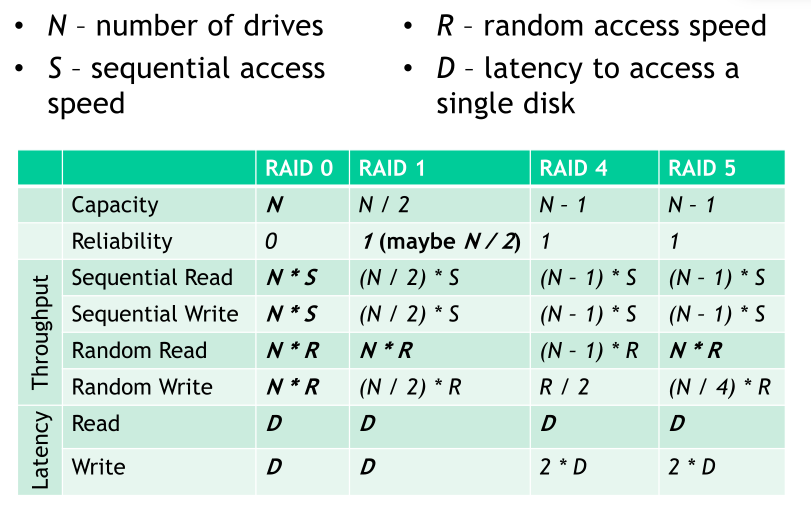
\includegraphics[width = \textwidth]{./images/raids.png}
					\end{figure}
					Where, more specifically:
					\begin{equation}
						\begin{cases}
							\text{Random transfer rate } R = \frac{transfer\, size}{time\, to\, access}\\
							\text{Sequential transfer rate } S = \frac{transfer\, size}{time\, to\, access}
						\end{cases}
					\end{equation}
					The difference between the two is the way the operations are actually issued on the disk.

		\section{Performance}
			\subsection{What is Performance?}
				Classic engineering question: how much did I do well? How do I measure, evaluate the goodness of my job? What's the most adapt figure of merit? How do I abstract enough from the reality in order to design the right solution (modeling problem)?
				
			\subsection{Approaches to Evaluation}
				Two main schools of thought:
				
				\paragraph{Measurements Based Techniques}
					Techinques as directly measuring the performances on the system, benchmarking it still "in beta" or prototyping approaches are based on the direct testing of the physical model or a copy of it.
					
				\paragraph{Model Based Techniques}
					Opposed to using the system itself to test performances, we can model it (build an abstract copy of it) and test that. Among these techniques are
					\begin{enumerate}
						\item Analytical, numerical tests
						\item Simulation
						\item Hybrid approaches
					\end{enumerate}
					This techniques are more "broad": they can test cases that it's possible that a bruta force approach as benchmarking never reach. 
					
			\subsection{Evaluating Performance through Queuing Networks}
				We'll use a model based approach to evaluate performance indexes. The model for us is queuing networks, classic distributed racing systems with scarce resources. These are usually represented as a set of services corredated with a queue to store clients. A client is served and then leaves the service. 
				
				\subsubsection{The Model}
					As said, a queuing network is composed by
					\begin{enumerate}
						\item Customers, or \emph{clients}, that need to use a service
						\item Service centers, that provide services. A service center is itself composed of
							\begin{enumerate}
								\item A buffer, the queue of arrivals
								\item A "server station" that provide the very server.
							\end{enumerate}
					\end{enumerate}
					\begin{figure}[H]
						\centering
						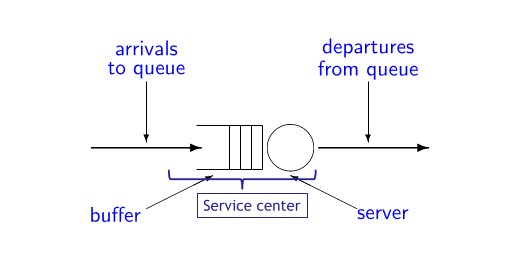
\includegraphics[width = \textwidth]{./images/queuingNetworks.png}
					\end{figure}
					
				\subsubsection{Parameters of the Model}
					To characterize our model, we usually quantify some of its aspects, such as
					
					\paragraph{Arrivals}
						Arrivals represent the clients of a system. In a network, they can come from either an external source, from another service station, or from the service station that they've just used (loop back arc).
						
					\paragraph{Services}
						Servers provide services. They can "hold" a client until the job is done, then they pass to the next element in the queue.
						
					\paragraph{Queue}
						The queues represent the buffer of clients before servers. When a client leaves the server, another one from the queue is selected \emph{according to the queuing policy}.
						
					\paragraph{Population}
						The population is the set of clients in the network. Ideally, each member is indistinguishable from the others; usually we can divide members in classes of members that all show the same behaviour. The behaviour of a member is characterized by several factors, as arrival rate, service demand, post service behaviour...
						
					\paragraph{Routing}
						The "place a client goes when is job has been served" is a parameter of the system, in particular is defined by the \emph{routing policy} of that system. Routing policies can be
						\begin{itemize}
							\item Probabilistic
							\item Channel based (like round robin)
							\item Queue based (like join-the-shortest-queu)
						\end{itemize}
			
			\subsection{The Performance Estimation Process}
				Once a model has been built (so in our case, a network of queuing processes) in order to evaluate the performance we have to parametrize the model itself and then estimate the performance indices. To do so, we must mathematically formalize how the model behaves: we can do such through the use of Operational Laws.\\
				Operational laws are basically equations that usually represents the the averaged behaviour of each system. Operational laws are based on observable variables, that can be "read" from the system. For example, given our model, we can without effort observe the variables
				\begin{itemize}
					\item The number of arrivals A
					\item The number of completions C
					\item The amount of time the system is busy B
					\item The average number of jobs in the system N
					\item The time span we used to observe the system T
					\item The visits to each station V
				\end{itemize}
				We can already derive some operational laws:
				\begin{center}
					\begin{tabular}{ | c | c |}
						\hline
						$ \lambda = \frac{A}{T} $ & Arrival rate \\
						$ X = \frac{C}{T} $ & Throughput \\
						$ U = \frac{B}{T} $ & Utilization time \\
						$ S = \frac{B}{C} $ & Mean service time\\
						\hline
					\end{tabular}
				\end{center}

				Notice that these laws can refer the whole system or the single service station. We direct our experiments on the model in order to have $\lambda = X$, also called "job flow balance" condition.\\
				From now on, if an property has a pedix, it's indicating that property (or operational law) of a particular service station or subsystem. Also, we need to introduce a new property if we're talking about single service station: this is $N$, the number of jobs in the \emph{whole service station}\footnote{so queuing + served}.
				
				\paragraph{Utilization Law}
					From literally one substitution we can derive the so called utilization law:
					\begin{equation}
						U_k = X_k \,\times\, S_k
					\end{equation} 
					This law expresses the "occupational fraction" of a station, so how much a station is busy. Expressed in words, it's the rate of arrival of requests times the time needed to carry out one of them. It's easy to notice how, if this value is greater than one, the queue will grow in time.
					
				\paragraph{Little Law}
					The Little's law (or result, or lemma) states
					\begin{equation}
						N = X \,\times\,R
					\end{equation}
					So \emph{the number of requests in the system is equal to the throughput multiplied by the average time R a request spends in the system}.
					
				\paragraph{Interactive Response Time}
					When measuring performance in an interactive system, we must also model in some way how the user behave in front of the system itself. To do so, we introduce \emph{think time} Z and we redefine N as $N = X \,\times\, (R + Z) $.

				\paragraph{Forced Flow Law}
					The FFL is another operational law that binds the the throughput of the entire system to the throughput of the single service stations.
					\begin{equation}
						X_k = V_k \,\times\, X
					\end{equation}
					Where $V_k$ is the visit count for the particular service station k, defined as $\frac{C_k}{C}$ so the fractions of completions of a single service station. Visit count is important when related to total completions: when $V_k$ is greater than one, the number of completions at system level corresponds to a higher number of visits to the single service station.\\
					
				\paragraph{Service Demand}
					The service demand represents the amount (in time) of service asked \emph{to a specific service station}. It's computed as
					\begin{equation}
						D_k = S_k \,\times\, V_k
					\end{equation}
					Remember: Service Time $\neq$ Residence Time. 
					
				\paragraph{Residence and Response Time}
					The response time $\tilde{R}$ is the time spent by a job in a service station, counting the queue time. The residence time instead is the time spent by a job in a service station \emph{during all system time}: so accounting for the loops and reiteration. The pretty straightforward relation is $R_k = V_k \,\times\, \tilde{R}$, that's the same relationship between Demand and Service Time. 
					
				\paragraph{General Response Time Law}
					The GRTL calculates the average response time for a job:
					\begin{equation}
						R = \sum_k (V_k \,\times\, \tilde{R_k}) = \sum_k (R_k)
					\end{equation}
					
				\subsubsection{SUMMARY}
					Ok so, we've seen some confusing stuff so far. Let's put all together in a nice table.
					\begin{center}
						\begin{longtable}{ | m{0.4\textwidth} || m{0.2\textwidth} | m{0.2\textwidth} | }
							\hline
							Name & Letter & Formula \\
							\hline
							\hline
							Number of arrivals & A & \textbackslash \\
							\hline
							Number of completions & C & \textbackslash \\
							\hline
							Busy time & B & \textbackslash \\
							\hline
							Average number of jobs in the system & N & \textbackslash \\
							\hline
							Observation time & T & \textbackslash \\
							\hline
							Visit to each station & V & \textbackslash \\
							\hline
							Think time & Z & \textbackslash \\
							\hline
							Arrival rate & $\lambda$ & $\frac{A}{T}$ \\
							\hline
							Throughput & X & $\frac{C}{T}$ \\
							\hline
							Utilization time & U & $\frac{B}{T}$ \\
							\hline
							Mean service time & S & $\frac{B}{C}$ \\
							\hline
							Utilization law & \textbackslash & $ U_j = X_k \,\times\, S_k$ \\
							\hline
							Little's law & \textbackslash & $ N = X \,\times\, R $ \\
							\hline
							Little's law, interactive response time & \textbackslash & $ N = X \,\times\,(R+Z) $ \\
							\hline
							Forced flow law & \textbackslash & $ X_k = V_k \,\times\, X $ \\
							\hline
							Service demand & \textbackslash & $ D_k = S_k \,\times\, V_k $ \\
							\hline
							General Response Time Law & \textbackslash & $ R = \sum_k(R_k) $ \\
							\hline
						\end{longtable}
					\end{center}

		\section{Performance Asymptotic Bounds}
			Performance bounds are the asymptotic values that our figures of merit can reach in a system. These can be useful in the modeling process to find the element that impact the most the performances, among the others the bottlenecks. Asymptotic analysis provides optimistic and pessimistic bounds on two major performance indexes: throughput X and response time R.
			
			\paragraph{Notation and Quantities}
				We'll focus on expressing X and R as functions of
				\begin{itemize}
					\item K $\rightarrow$ number of service centers
					\item D $\rightarrow$ sum of all the service demands at the centers
					\item $D_{max}$ $\rightarrow$ largest service demand at a single center
					\item Z $\rightarrow$ average think time for interactive systems
				\end{itemize}
				We'll analize
				\begin{itemize}
					\item Optimistic scenarios, where we search X's upper bound and R's lower bound
					\item Pessimistc scenarios, viceversa: throughput lower bound and maximum values of response time
				\end{itemize}
			
			\subsection{Tables of Formmulae}
				Bounds for throughput
				\begin{longtable}{ m{0.1\textwidth} | m{0.45\textwidth} | m{0.45\textwidth} |}
					& Open Systems & Closed Systems \\
					\hline
					Light Load & \multirow{2}{0.3\textwidth}{ 
						\begin{equation}
							X(\lambda) \leq \frac{1}{D_{max}}
						\end{equation}
					} &  
						\begin{equation}
							\frac{N}{ND + Z} \leq X \leq \frac{N}{D + Z}
						\end{equation}
					\\
					Heavy Load & & 
						\begin{equation}
							\frac{N}{ND + Z} \leq X \leq min(\frac{N}{D + Z}, \frac{1}{D_{max}})
						\end{equation}
					\\
					\hline					
				\end{longtable}
				Bounds for response time:
				\begin{longtable}{ m{0.1\textwidth} | m{0.45\textwidth} | m{0.45\textwidth} |}
					& Open Systems & Closed Systems \\
					\hline
					Light Load & \multirow{2}{0.3\textwidth}{ 
						\begin{equation}
							R \geq \frac{1}{D_{max}}
						\end{equation}
					} & \multirow{2}{0.3\textwidth}{
						\begin{equation}
							max(D_{max}, ND_{max}-Z) \leq R \leq ND
						\end{equation}
					}
					\\
					Heavy Load & & \\
					\hline					
				\end{longtable}

			\subsection{SUMMARY}	
				\begin{figure}[H]
					\centering
					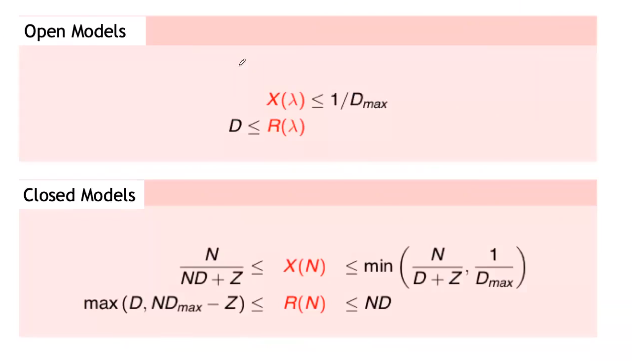
\includegraphics[width = \textwidth]{./images/superSummary2.png}
				\end{figure}
				
	\clearpage \part{Dependability}
		\section{Probabilistic approach}
			Dependability represents the \emph{availability performance} of a system. It encompasses 
			\begin{itemize}
				\item Reliability
				\item Availability
				\item Maintainability
			\end{itemize}
			
			Dependability is approached with a statistical/probabilistic POV due to the high human component in it.\\
			Two functions describes the system: F(t) and f(t), respectively the cumulative function and the fault probabilistic distribution. The former represents the \emph{unreliability} of the system analyzed. So, we can define $R(t) =  1 - F(t)$ as the reliability function.\\
			Probabilistics recall:

			\begin{align}
				f(t) \rightarrow \text{ probabilistic distribution of failure}\\
				F(t) = \int_{0}^{t}f(t)dt \rightarrow \text{ cumulative function, unreliability}\\
				R(t) = 1 - F(t) \rightarrow \text{ reliability function}
			\end{align}

			To be noticed: the function $F(t_i)$ represents the probability that component $i$ is working at time $t_i$ \emph{knowing it was working at time 0}. This is to be taken in mind to make a comparison with the failure rate.\\
			From this we can define the Mean Time To Failure for a component (that's the expected value):
			\begin{equation}
				\begin{cases}
					MTTF = \int_0^{\infty}t \cdot f(t)dt\\
					MTTF = \int_0^{\infty}R(t)dt
				\end{cases}
			\end{equation}
			We can also define the failure rate (mathematically, the conditioned probability):
			\begin{equation}
				\lambda(t)dt = F(t < T \leq t+dt \,\vert\, T > t)
			\end{equation}
			So the failure rate represents the probability of failure \emph{assuming the component was working the instant before}. This function can be seen as the number of failures in a given interval.
			
			\subsection{Failure Rate}
				Type of malfuntioning:
				\begin{itemize}
					\item Fault: physical defect or software bugs.
					\item Error: program incorrectness that can result from a fault.
					\item Failure: nonperformance of some actions that were expected. They can be result of an error.
				\end{itemize}
				
				\paragraph{Properties of the failure rate}
					Probabilistically, failure rate is
					\begin{equation}
						\lambda(t)dt = F(t < T \leq t+dt \,\vert\, T > t)
					\end{equation}
					So we can derive
					\begin{equation}
						\lambda(t)dt = \frac{P(t < T < t + dt \cap T > t)}{P(T > t)}
					\end{equation}
					From the definition of combined probability, with P as probability. Given
					\begin{equation}
						P(t < T < t+dt) \cap P(T > t) = P(t < T < t+dt)
					\end{equation}
					We obtain
					\begin{equation}
						\lambda(t)dt = \frac{f(t)dt}{R(t)} = \frac{dF(t)}{R(t)} = -\frac{dR(t)}{R(t)}
					\end{equation}
				
				\paragraph{Reliability as Weibull}
					Failure rate $\lambda(t)$ function has a peculiar function shape: a \emph{bathub} (or long U) shape. The failure rate is high in the starting period and decreases (infant mortality effect) to the costant level during the useful lifetime (costant probability of failures) and it raises again at the end (wear out period).\\
					
					In fact, reliability follows the \emph{Weibull distribution} so definied: $y(x) = e^{-(\frac{x}{\alpha})^{\beta}}$. So (due to the $\lambda(t) = f(t) / R(t)$ relation) we obtain
					\begin{equation}
						\lambda(t) = \frac{\beta}{\alpha}(\frac{t}{\alpha})^{\beta - 1}
					\end{equation}
					
				\paragraph{Reliability as exponential}
					We can also model the reliability as an exponential function (so $R(t) = e^{-\lambda t}$) we than obtain
					\begin{equation}
						\begin{cases}
							F(t) = 1 - e^{-\lambda t} \\
							f(t) = \lambda e^{-\lambda t} \\
							MTTF = \int_{0}^{\infty} t\cdot \lambda e^{-\lambda t} dt = \frac{1}{\lambda} \,\Rightarrow\, \lambda = \frac{1}{}
						\end{cases}
					\end{equation}
					So we can express the reliability as function of MTTF: $R(t) = e^{-\frac{t}{MTTF}}$. And we all know that in certain conditions (like $\frac{t}{MTTF} << 1$) an exponential function can be approximated to a linear function.

			\subsection{System level reliability}
				We can model the system relibility mainly with RBDs: Reliability Block Diagram. These simply outline the operational dependency between components. The main assumption of the RBD is that the failures are \emph{indipendent}, that implies that are no "cascading failures".\\
				General formulae for the Reliability of systems:
				\begin{equation}
					\begin{cases}
						\text{Serial components: } R_s(t) = \prod_{i=1}^{n}R_i(t)\\
						\text{Parallel components: } R_p(t) = 1 - \prod_{i=1}^{n} (1-R_i(t))
					\end{cases}
				\end{equation}

				\paragraph{System's MTTF}	
				We can redefine the mean time to failure to cover the complex systems, keeping in mind the two configurations we use: serial or parallel components.
				\begin{equation}
					\begin{cases}
						\text{Serial components: } MTTF_s = \frac{1}{\sum_{i = 1}^{n}(\frac{1}{MTTF_i})} \\
						\text{Serial \emph{identical} components: } MTTF_{ss} = \frac{MTTF}{n} \\
						\text{Parallel components: } MTTF_p = \sum_{i = 1}^{n}(MTTF_i) - MTTF_s \\
						\text{Parallel \emph{identical} components: } MTTF_{pp} = MTTF_i * (\sum_{i = 1}^{n - 1} (\frac{1}{n - i}))
					\end{cases}
				\end{equation}

				\paragraph{Disclaimer}
				MTTF is an \textit{integral measured value}, it must be handled with care when the number of components and links grow. The perfect workflow is to fix unreliability, then calculate reliability\footnote{additional step, not always needed}, derive to obtain $f(t)$, then \textit{at the end} derive MTTF as expected value of $f(t)$.

			\subsection{Availability}
				Introducing MTTR, Mean Time To Repair. This represents the average time required to replace a failed component and "bring the system back up" after a failure. It can be the restart time (for software module) or the replace time (for an hardware component).\\
				Another interval to be taken into consideration when talking about availability is the Mean Time Between Failure, that's just the sum of $MTTF + MTTR$. Availability is defined as the probability of a system to be up and running at a given istant. So $Av = \frac{MTTF}{MTBF}$ that corresponds to
				\begin{equation}
					Availability = \frac{MTTF}{MTTF+MTTR}
				\end{equation}
				The slight difference between availability and reliability takes into consideration the repairing of a system in the case it goes down. The availability function is calculated with \emph{the same identical formulas} used to calculate the reliability for parallel and serial components:
				\begin{equation}
					\begin{cases}
						\text{Serial components: } A_s = \prod_{i = 1}^n A_i \\
						\text{Parallel components: } A_p = 1 - \prod_{i = 1}^n (1 - A_i)
					\end{cases}
				\end{equation}
				Talking about MTTF when taking into consideration that components can be \emph{repaired} must be carefully handled: for example, if a parallel system has \emph{interleaving} failures, it never fails enitrely. A way of calculating MTTF for repairable system consists in inverting formula (9), obtaining
				\begin{equation}
					MTTF = \frac{Av*MTTR}{1-Av}
				\end{equation}
\end{document}
